\documentclass[a4paper]{article}
\usepackage[T1]{fontenc}
\usepackage[utf8]{inputenc}
\usepackage{natbib}
\usepackage{hyperref}
\usepackage{wrapfig} % place figure to the left
\usepackage{multirow} % context example table
\usepackage{graphicx} % include the map
\usepackage[outline]{contour} % contour place names in the cosine similarity figure
\usepackage[dvipsnames]{xcolor} % colour-code the groups (has to come before tikz)
\usepackage[geometry]{ifsym} % shape-code the groups
\usepackage[section]{placeins} % don't let the graphics/tables move past sections
\usepackage{tipa} % IPA
\usepackage{amsmath} % formulae
\usepackage{mathtools} % displaystyle in formulae with cases
\usepackage{forest} % (non-dendrogram) trees
\usetikzlibrary{decorations.pathreplacing} % draw braces in tikz figures
\usepackage{standalone} % import figures
\usepackage{changepage} % adjust text width
\usepackage{parskip} % proper paragraphs, no indentation
\usepackage{showframe} % TODO remove
\usepackage[margin=3cm]{geometry}

% TODO make the hues match those of the map
\def\upper{\color{red}\FilledBigTriangleUp}
\def\central{\color{Dandelion}\FilledBigSquare}
\def\dutch{\color{ForestGreen}\FilledBigCircle}
\def\ingv{\color{Blue}\BigCircle}

\title{Clustering Dialect Varieties Based on Historical Sound Correspondences}
\author{Verena Blaschke}
\date{\today}

\begin{document}

\begin{titlepage}
\begin{center}

\vspace*{.15\textheight}

{\Large Bachelor's Thesis}
\vspace{2em}

\hrule
\vspace{0.6cm}
{\huge\bfseries
Clustering Dialect Varieties Based on Historical Sound Correspondences
}\\[0.7cm] 
\hrule
\vspace*{.05\textheight}
 
\begin{minipage}[t]{0.4\textwidth}
\begin{flushleft} 
{\large
\textit{Author}\\
Verena Blaschke}\\
\href{mailto:verena.blaschke@student.uni-T\"{u}bingen.de}{\textit{verena.blaschke@student.uni-T\"{u}bingen.de}}\\
\end{flushleft}
\end{minipage}
\begin{minipage}[t]{0.4\textwidth}
\begin{flushright}
{\large
\textit{Supervisor}\\
Dr. Çağrı Çöltekin}\\
\href{mailto:ccoltekin@sfs.uni-T\"{u}bingen.de}{\textit{ccoltekin@sfs.uni-T\"{u}bingen.de}}\\
\end{flushright}
\end{minipage}\\

\vfill

A thesis submitted in partial fulfillment\\
of the requirements for the degree of\\[2mm]
{\large Bachelor of Arts}\\
in\\[1mm]
{\large International Studies in Computational Linguistics}

\vspace*{.1\textheight}

{\large Seminar für Sprachwissenschaft\\
Eberhard Karls Universität Tübingen

\vspace{1em}
August 2018}
\end{center}
	
\end{titlepage}




\pagenumbering{gobble}
% TODO abstract
\newpage
\tableofcontents
\newpage
\listoftables
\listoffigures
\newpage
% TODO Eigenständigkeits- bzw. Antiplagiatserklärung  

\pagenumbering{arabic}


\section{Introduction}

% --- on clustering dialects and determining relevant features ---

clustering dialects and determining relevant features

\citet{prokic2012detecting}


\citet{heggarty2010splits} created a NeighborNet for Germanic languages, based on pronunciation differences between modern varieties. 
~conclude~ that this works because the pronunciation differences implicitly include information on sound changes that were not shared by all varieties

\citet{prokic2013combining}: judging regularity of correspondences via contingency table

% --- on historical sound correspondences ---

historical sound correspondences

% \citet{kondrak2009identification}
% https://pdfs.semanticscholar.org/d2ea/1dbe1a81f60f99dab04dffc957622b8cb9f2.pdf
% https://www.clips.uantwerpen.be/~gillis/pdf/20040107.9620.cslfinal.pdf
% https://www.aclweb.org/anthology/J/J96/J96-4003.pdf

% --- on BSGC ---

Bipartite spectral graph co-clustering

introduced in \citet{dhillon2001co-clustering}

introduced as a method for dialect clustering in \citet{wieling2011bipartite}

\citet{wieling2013analyzing} applied this method for clustering British English dialects and compared the results to clusters obtained via PCA
 
\citet{montemagni2013synchronic} applied this method to Tuscan dialects and used left and right contexts for the sound segments

\citet{zha2001bipartite} introduced a similar (the same??) method as Dhillon at the same time, in another journal

% These algorithms and related ones were investigated by \citet{kluger2003spectral} for their use in bioinformatics as well (co-clustering genes and phenotypes).

This thesis is structured as follows:
We begin by introducing the data in section~\ref{sec:data}.
Then, in section~\ref{sec:cwg},
we give a brief introduction to continental West Germanic doculects,
proposed groupings of doculects belonging to that group of doculects
and the problems associated with doing this.
In section~\ref{sec:methods}, we explain our methodology for
aligning the data and extracting sound correspondences,
and then for the two approaches to clustering the data that we employ,
and explain how we rank the sound correspondences.
We present the results in section~\ref{sec:results}
and discuss them in section~\ref{sec:discussion}.

% \newpage
\section{Data}
\label{sec:data}

We work with phonetically transcribed data from
continental European West Germanic (herafter: CWG) dialects and standard languages
(hereafter referred to as doculects).
The data we work with are taken from the Sound Comparisons project
lead by \citet{heggarty2018sound}, who compiled IPA transcriptions of word lists
in a range of Germanic doculects.

From this database,
we used 110 cognate sets from 20 modern CWG doculects
and a reconstructed version of Proto-Germanic.
\footnote{
The Sound Comparisons project does not state
the theoretical basis for the Proto-Germanic reconstruction.
According to the project website,
the reconstruction probably is close to
a variant of the language spoken in around 500 BCE
in Southern Scandinavia.
}
Of the modern doculects, two are identified as standard languages
in the database (Dutch spoken in the Netherlands and Belgium
\footnote{
Hereafter referred to as ``Std. Dutch (NL)'' and ``Std. Dutch (BE)'', respectively.
}),
the rest as local vernaculars.
The modern doculects are from locations in the
Netherlands, Belgium, Luxembourg, (along the Western border of) Germany,
France (Alsace), Switzerland, Liechtenstein, Austria (Lake Constance), and Italy (South Tyrol).
Figure~\ref{fig:map} provides an overview of these locations.
The legend is explained in section~\ref{sec:cwg}.

For the phonetic alignment step (see section~\ref{subsec:msa}),
we used 14 additional doculects that are Germanic but not continental West Germanic. 
To control for transciber bias,
we only worked with doculects that share the same transcriptor,
Warren Maguire.
The transcriptions of the modern doculect data
are narrow transcriptions;
that of the Proto-Germanic reconstruction appears to be broader.
\footnote{
For instance, the Proto-Germanic data include no suprasegmentals.
}

We excluded one CWG doculect that covered only 35 concepts. % Schaeddel (Frisian)
The Proto-Germanic data cover all 110 concepts; each of the modern doculects covers at least 103 concepts, and each concept is covered by at least 17 modern doculects.
In total, we have 2181 sequence alignments between Proto-Germanic and modern CWG doculects.

note on inflected forms

\begin{figure}[h]
\centering
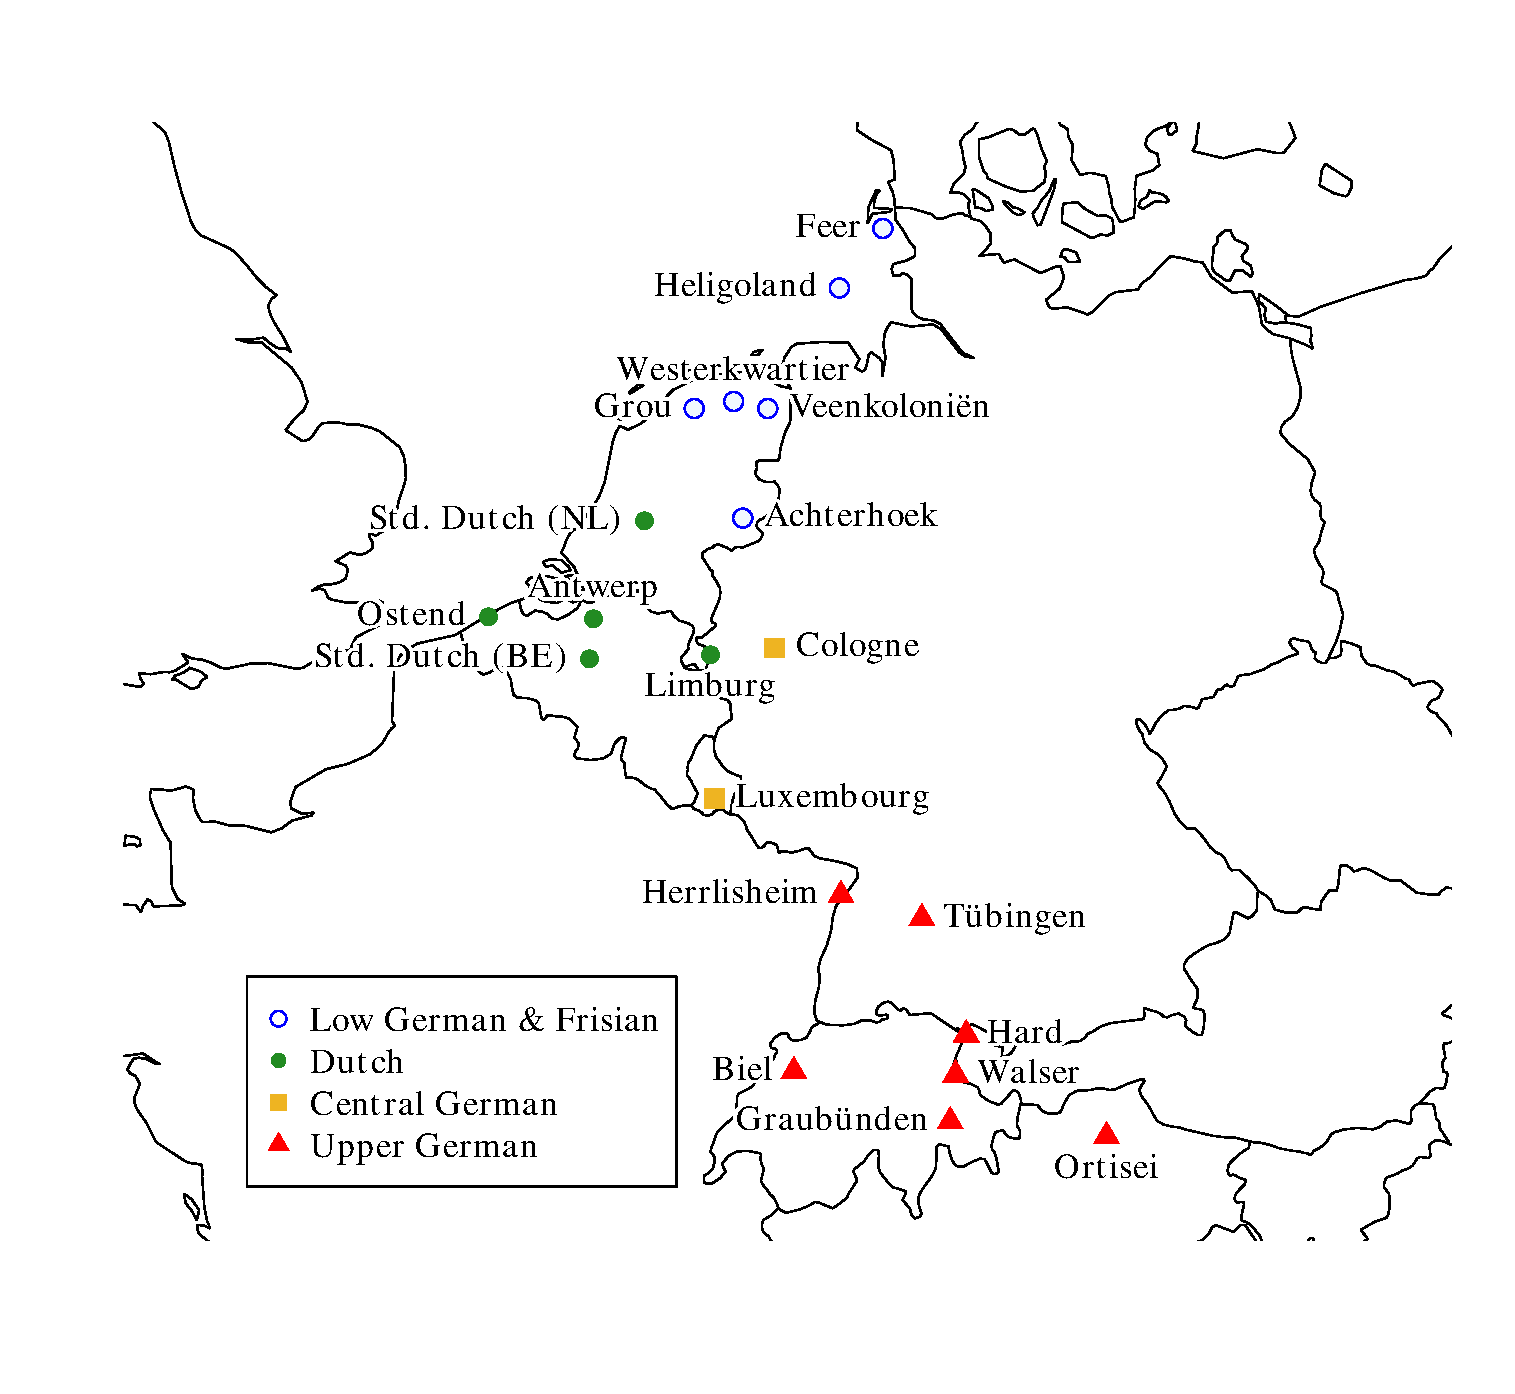
\includegraphics[width=\textwidth]{figures/map.pdf}
\caption{Locations of the modern continental West Germanic doculects we worked with.}
\label{fig:map}
\end{figure}


% \newpage
\section{Continental West Germanic}
\label{sec:cwg}

Grouping the CWG doculects provides a challenge
that has been taken up many times, with different results.

Even the classification of West Germanic
as its own branch of Germanic is controversal,
though generally accepted
(c.f. \citet{voyles1971problem}; \citet[pp. 7-8]{harbert2007germanic}; \citet{ringe2012cladistic}). % \citet[p. 404]{krogh1996stellung}

Within the CWG dialect continuum, it gets even more complicated and contested.
CWG doculects are very similar to one another and closely related.
These similarities do not only exist because of genetic relatedness
but also--enabled by the geographic proximity--mutual influences
\citep[p. 8]{harbert2007germanic}.
This position is also reflected in Figure~\ref{fig:cwg_harbert},
which shows a proposed division of CWG doculects
into three main groups: North Sea Germanic (including Frisian and Low German),
Franconian (including Dutch and High Franconian),
and Alpine Germanic (including Alemannic and Bavarian).
It presents High German as the result of the convergence
of High Franconian, Alemannic and Bavarian.

\begin{figure}[b]
\centering
\includestandalone[width=\textwidth]{figures/harbert}
\caption{
The internal structure of continental West Germanic
based on \citet[p. 8]{harbert2007germanic}.
}
\label{fig:cwg_harbert}
\end{figure}

%TODO Heggarty splits waves

\citet{hammarstroem2018glottolog}, whose language catalogue
contains strictly hierarchical categorizations, % TODO source??
gives an entirely tree-like classification of the CWG doculects,
as shown in Figure~\ref{fig:glottolog}.
This classification is based on the work by \citet{stiles2013pan-west}
and, as the previous figure, \citet{harbert2007germanic}.
We include it here since the output of the clustering methods
is also strictly hierarchical.

\begin{figure}[h]
\begin{adjustwidth}{-3cm}{-3cm}
\centering
\scalebox{0.8}{
\documentclass{standalone}
\usepackage[utf8]{inputenc}
\usepackage{forest}
\begin{document}
\begin{forest}
short/.style={l sep=1mm},
for tree={
  parent anchor=south, 
  child anchor=north,
  align=center, % necessary for intra-node linebreaks
  l sep=3cm, % level
  s sep=0.5mm, % sibling
%   inner sep=0.2mm
}
[West Germanic
  [North Sea Germanic
    [Anglo-Frisian, short
    [Frisian
        [Western\\Frisian\\\textit{Grou}]
        [Northern\\Frisian
            [Ferring\\\textit{Feer}]
            [Helgoland\\\textit{Heligoland}]
        ]
    ]
    ] 
    [Alts\"{a}chsisch\\{[Old Saxon]}, short
    [Middle-Modern\\Low German, short
    [Low German
        [Achter-\\hoeks\\\textit{Achterhoek}]
        [Ost-\\friesisch-\\Groningisch, short  % TODO translation
        [Gronings
            [Veenkolonials\\\textit{Veenkoloni\"{e}n}]
            [Westerwolds\\\textit{Westerkwartier}]
        ]
        ]
    ]
    ]
    ]
  ]
  [Franconian
    [Low Franconian, short
    [Macro-Dutch, short
    [Modern Dutch
        [Dutch\\\textit{Std. Dutch}\\\textit{(NL)}]
        [Vlaams\\\textit{Std. Dutch}\\\textit{(BE)}
            [Ostvlaams\\\textit{Ostend}]
            [Antwerps\\\textit{Antwerp}]
            [Limburgs\\\textit{Limburg}]
        ]
    ]
    ]
    ]
    [High Franconian
        [German, short
        [Alsatian\\\textit{Herrlisheim}]
        ]
        [Middle\\Franconian
            [Luxem-\\bourgish\\\textit{Luxembourg}]
            [Ripurarian, short
            [Kölsch\\\textit{Cologne}]
            ]
        ]
    ]
  ]
    [High German, short
    [Middle-Modern\\High German, short
    [Modern\\High German, short
    [Alpine Germanic
    [Alemannic
        [Swiss\\German
            [Basel\\\textit{Biel}]
            [Low\\Alemannic\\\textit{Hard}]
            [Graubenden-\\Grisons\\\textit{Graub\"{u}nden}]
        ]
        [Swabian\\\textit{T\"{u}bingen}]
        [Walser\\\textit{Walser}]
    ]
    [Bayerisch\\{[Bavarian]}
    [Cimbrian\\\textit{Ortisei}]
    ]
  ]
  ]
  ]
  ]
]
\end{forest}
\end{document}

}
\end{adjustwidth}
% \includestandalone[width=\textwidth]{figures/glottolog}
\caption
[
The full classification tree (up to West Germanic) for the modern doculects we used,
as defined by \citet{hammarstroem2018glottolog}.
]
{
The full classification tree (up to West Germanic) for the modern doculects we used,
as defined by \citet{hammarstroem2018glottolog}.
The names of the modern doculects are dispayed in italics.
}
\label{fig:glottolog}
\end{figure}

\citet[pp. 72-80]{nielsen1989germanic} gives an overview of the history of attempting to divide the West Germanic dialects into subgroups with the associated criteria (phonological, morphological, lexical, and/or extra-linguistic) and criticisms.

On the other hand, more recently, % TODO than what?
interactions between dialects and standard languages
have influenced the dialect landscape
\citep{coetsem1992interaction}.
\citet{kremer1990einfuehrung} found that in Germany and in the Netherlands
(but not in Switzerland), dialects tend to become closer to the standard languages,
with the result of state or standard language borders tending to act as dialect borders.
(They also found that Low German dialects tend and CWG spoken in Non-Germanic (e.g. francophone) regions tend to be replaced by the standard language instead.)

\subsection{North Sea Germanic}

\citet{stiles2013pan-west} posits that
the most significant division of West Germanic varieties is
the split into Ingv\ae{}onic (that is, North Sea Germanic) varieties
and non-Ingv\ae{}onic varieties.
This split is also supported by, e.g., \citet[p. 7]{harbert2007germanic}, \citet[pp. 117--123]{sonderegger1979grundzuege}, and \cite{auwera2017germanic}.
What is more complicated is the definition of which doculects Ingv\ae{}onic consists of:
% \citet{stiles2013pan-west} defines this group
% as Frisian, English, and ``to a certain extend, Old Saxon'' (i.e., Low German),
% whereas \citet[pp. 7, 17]{harbert2007germanic} defines it
% as Frisian, English, and Old Saxon,
% while noting that Dutch has also been influenced by the Ingv\ae{}onic languages.
% \citet[pp. 71, 117--123]{sonderegger1979grundzuege} classifies Ingv\ae{}onic
% as Frisian, English, Low German, and (having become a part of this group more recently) Dutch,
% while \citet{auwera2017germanic} define Ingv\ae{}onic as Frisian, English, and Dutch.
\begin{itemize}
\item 
\citet{stiles2013pan-west} defines this group
as Frisian, English, and ``to a certain extend, Old Saxon'' (i.e., Low German),

\item
\citet[pp. 7, 17]{harbert2007germanic} defines it
as Frisian, English, and Old Saxon,
while noting that Dutch has also been influenced by the Ingv\ae{}onic languages,

\item
\citet[pp. 71, 117--123]{sonderegger1979grundzuege} classifies Ingv\ae{}onic
as Frisian, English, Low German, and (having become a part of this group more recently) Dutch, % TODO elaborate on 'more recently'

\item
\Citet{auwera2017germanic} define Ingv\ae{}onic as Frisian, English, and Dutch.
\end{itemize}

The distinct properties of the Ingv\ae{}onic subgroup
concern mostly inflection and pronouns
(\citet{stiles2013pan-west}; \citet[pp. 7-8]{harbert2007germanic}),
although \citet{stiles2013pan-west} also lists some phonological characteristics:
``backing of long and short *\textit{a} before nasals[...];
fronting of long and short *\textit{a};
and palatalization of velar consonants''.

Following the categorization by \citet{harbert2007germanic}, % TODO reason
we can divide the modern doculects from our dataset as follows:

\begin{itemize}
\item 
\textbf{Ingv\ae{}onic:}
Feer, Heligoland, Grou,
Westerkwartier, Veenkoloni\"{e}n, Achterhoek

\item
\textbf{Non-Ingv\ae{}onic:}
Std. Dutch (NL), Std. Dutch (BE), Ostend, Antwerp, Limburg,
Herrlisheim, Luxembourg, Cologne,
Ortisei, T\"{u}bingen, Walser, Biel, Hard, Graub\"{u}nden.
\end{itemize}

In Figure~\ref{fig:map}, the Ingv\ae{}onic doculects
are marked with blue, non-solid circles.
A split similar to the one proposed by \citet{sonderegger1979grundzuege}
is part of the following section.

\subsection{Results of the High German Sound Shift}

A very important development for the CWG doculects,
especially High German, is the High German sound shift.
\footnote{
The term \textit{High German sound shift} has been used both
to only describe the High German consonant shift,
and to describe the consonant shift and sound shifts concerning
the High German vowel system.
We use it here with the former meaning.
}
Summarizing \citet[pp. 47--48]{harbert2007germanic}
and \citet[pp. 62--64]{koenig2015dtv},
we can outline the High German sound shift as follows:

The voiceless (aspirated)
\footnote{
Aspiration is not marked in the reconstructed version of Proto-Germanic
we worked with.
}
Germanic stops (/*p, *t, *k/)
underwent lenition and shifted into affricates or fricatives.
(Typically, these stops developed into fricatives in postvocal positions,
and into affricates in word-inital or postconsonantal positions,
and /*t/ changed more commonly than /*p/,
which in turn changed more commonly than /*k/.)
To balance this out,
the voiced Germanic stops (/*b, *d, *g/) on the other hand
developed into their voiceless (and aspirated) counterparts.

Generally, these changes are pronounced
in the Southern CWG area, and did not take place in the North
\cite[p. 33]{noble1983modern}
\footnote{
It is therefore generally assumed that the locations
from which these changes spread are in the Southern CWG area,
although there are also some controversies surrounding this
\citep[pp. 155--181]{goblirsch2005lautverschiebungen}.
}.
In between, there are many doculects
that only partially realized the High German sound shift,
with some of the changes only applying to individual words
\citet[p. 63]{koenig2015dtv}.

Based on this, there is a common split
of CWG doculects spoken in Germany into three groups:
Upper German doculects, which exhibit lenition for
all three voiceless stops almost completely
(except for sometimes /*k/ $>$ /(k)x/),
Central German doculects, which show a
partial development of the High German sound shift,
and Low German doculects,
which were not influenced by the High German sound shift
\citep[pp. 33, 55]{noble1983modern}.

This division is performed based on
the presence or absence of this shift in individual words.
The pronunciation boundaries (isoglosses) for such words
sometimes appear tightly bundled together,
although such bundles can also fan out such that a region
contains a continuum of very subtle dialect differences,
as is the case with the so-called Rhenish Fan at the Western part
of the boundary (or transition zone) between Low and Central German
\citep[pp. 63, 138, 141]{koenig2015dtv}.

We base the following classification of
the CWG doculects we worked with
on a map by \citet[pp. 230-231]{koenig2015dtv}:
\footnote{
% TODO refine or remove
Central German is delimited % TODO word choice
to the North (Low German) with an isogloss bundle containing
'ik/ich, maken/machen, Dorp/Dorf'...
}

\begin{itemize}
\item
\textbf{Low German, Dutch, and Frisian:}
Westerkwartier, Veenkoloni\"{e}n, Achterhoek,
Feer, Heligoland, Grou,
Std. Dutch (NL), Std. Dutch (BE), Ostend, Antwerp, Limburg.

\item
\textbf{Central German:}
Cologne, Luxembourg.

\item
\textbf{Upper German:}
T\"{u}bingen, Herrlisheim,
Biel, Graub\"{u}nden, Walser, Hard, Ortisei.
\end{itemize}

Figure~\ref{fig:map} shows this division:
Low German, Dutch and Frisian are marked with (solid green and non-solid blue) circles,
Central German with yellow squares, and Upper German with red triangles.

This division also matches the intra-database grouping by \citet{heggarty2018sound}
(who additionally split up the last group into
Low German on the one hand,
and Frisian, Dutch, and Flamish on the other).

% \newpage
\section{Methods}
\label{sec:methods}

\subsection{Multiple Sequence Alignment}
\label{subsec:msa}

In order to extract sound correspondences,
we need to align the sound sequences corresponding to each concept first.
We carry out alignment based on data from
all the investigated doculects at once using multiple sequence alignment.
Using multiple sequence alignment instead of carrying out
pairwise alignments between the modern data and the reference data
makes it possible to carry out the alignment
based on patterns found in commonalities between the modern doculects as well.
Because of this, we use all of the Germanic data
we extracted from the Sound Comparisons project
instead of only the CWG doculects and Proto-Germanic.

We use a library-based version \citep{notredame2000t-coffee:} of the progressive multiple sequence alignment method \citep{thompson1994clustal}.
For each concept:

\begin{enumerate}
\item
Divide the phonetic representation of each word into an array of sound segments.
These sound segments are typically single IPA tokens (including diacritics), but we use multi-token segments for affricates, diph- and triphthongs, and geminates.
\footnote{
Allowing multi-token segments is different from
the method employed by, e.g., \citet{wieling2010hierarchical}.
They neither allowed multi-token segments nor did they add contextual information
(see \ref{subsec:corres}),
but they remark on a common alignment $\emptyset$:[\textesh],
which commonly appears after [t]:[t].
We opt instead to interpret affricates as single segments with
the result of correspondences such as [t]:[\texttoptiebar{t\textesh}].

}

\item
Create alignments for all possible binary sequence combinations.
These alignments are created using the algorithm from \citet{needleman1970general},
with a scoring scheme based on the sound classes introduced by \citet{list2012sca}.
All segment alignments from this step are stored in a library,
each associated with a weight reflecting its relative frequency.
% TODO. in how far does it reflect probable sound class changes in the LingPy implementation (vs. relative frequency)

\item
Use the binary calculations to create a distance matrix between the sequences.
Convert the distance matrix into a tree using the UPGMA method \citep{sokal1958statistical}.

\item 
Progressing from the tips of the tree to the root,
consecutively join the alignments meeting at branchings,
until (at the root) all alignments have been consolidated into one alignment table.
Alignments are merged using the library created in the first step.
\end{enumerate}

We use the LingPy library for Python \citep{list2018lingpy} to perform these steps.
Table~\ref{tab:msa} shows an excerpt from the multiple sequence alignment for the concept ``cold''.

\begin{table}[h]
\begin{center}
\begin{tabular}{l|llllll}
\hline
Doculect       & \multicolumn{6}{l}{Sound segments} \\ \hline
Proto-Germanic  & k    & a    & l   & d    & a  & z  \\
Westerkwartier & k\textsuperscript{h}   & o    & \textltilde   & t\textsuperscript{h}   & -  & -  \\
Luxembourg     & k\textsuperscript{h}   & a\textlengthmark   & l   & -    & -  & -  \\
Biel           & \textchi    & \textscripta\textupsilon   & -   & t    & -  & -  \\
Walser         & x    & a\textlengthmark    & l   & t    & -  & -  \\
Ortisei        & k\textsuperscript{h}   & \textopeno    & l   & \texttoptiebar{ts}  & -  & - \\ \hline 
\end{tabular}

\end{center}
\caption{An excerpt from the aligned sequence table for the concept ``cold''.}
\label{tab:msa}
\end{table}

\subsection{Sound Correspondence Extraction}
\label{subsec:corres}

After performing sound segment-wise alignment,
we extract sound correspondences between each
modern doculect and Proto-Germanic from the alignment table.
We use straightforward segment-to-segment correspondences
as well as correspondences that include contextual information:

\begin{itemize}
\item
\textbf{No context}:
These are simple segment-to-segment correspondences.

\item
\textbf{Simple context}:
We (separately) add information about the
left and right single-segment context,
stating whether the context is a consonant or vowel. 
This can only be performed when the context in question is of
the same type for both Proto-Germanic and the modern doculect.

\item
\textbf{Sound class-based context}:
This is similar to the previous category,
but we give more fine-grained information about consonants and vowels.
We use the sound classes introduced by \citet{list2012sca},
which discern between fifteen consonant groups and sixteen vowel groups.
We do not include information on word boundaries or gaps here,
as it would be identical to the word boundary- or gap-related information
included in the correspondences with simple contextual information.
% TODO mention cases where SCA was useful in other applications

\item
\textbf{Word boundary-based context}:
This category applies when the context is a word boundary.

\end{itemize}

% TODO check montemagni. also ref them here
Table~\ref{tab:context} provides an overview
of the different context types, as found in the data.
IPA characters with diacritics are classified
like their diacritic-less counterparts,
and diphthongs/triphthongs are classified
according to the first character in the sequence.
Table~\ref{tab:corres} shows the sound correspondences
that can be inferred for the aligned segments
from Proto-Germanic and Ortisei German for the alignment
shown in Table~\ref{tab:msa}.

We ignore gap-gap alignments,
as they do not contain information on correspondences
between Proto-Germanic and the modern doculect in question,
only about an inserted sound segment in one or more other doculects.
Furthermore, we treat insertions and deletions
that LingPy flags as swaps (metathesis) as normal insertions/deletions,
as such cases only happen for 3 of the 111 concepts.

For each doculect, we ignore sound correspondences
that occurless than three times across all concepts
to reduce the effect misalignments can have. 

After extracting the sound correspondences for
all modern doculects, we have a doculect-by-correspondence
matrix storing the absolute frequencies of the sound correspondences.

\begin{table}[]
\begin{tabular}{llll}
Context type & Abbrev. & Definition & Corresponding IPA characters in our data\\\hline
Word boundary & \# & word boundaries & \\[3mm]

\multirow{2}{*}{Simple context} & cons & consonants & \\
    & vow & vowels & \\[3mm]

\multirow{18}{*}{\begin{tabular}[c]{@{}l@{}}Sound class-\\ based context\end{tabular}}
    & A & unrounded open vowels          & a, \textscripta \\ % reported as 'unrounded *back* vowels' in List2012 
    & B & labial/labiodental fricatives  & f, \texttoptiebar{pf}, v, \textphi, \textbeta\\
    & C & dental/alveolar affricates     & \texttoptiebar{dz}, \texttoptiebar{ts}, \texttoptiebar{t\textesh}\\ % not as context
    & D & dental fricatives              & \dh, \texttheta\\ % not as context
    & E & unrounded mid vowels           & e, \ae, \textturna, \textschwa, \textepsilon, \textrevepsilon, \textturnv \\
    & G & velar/uvual fricatives         & x, \textchi, \textgamma \\ % gamma not used as context
    & H & laryngeals                     & h, \texthth, \textglotstop \\ % only h used as context
    & I & unrounded close vowels         & i, \i \\
    & J & palatal approximants           & j \\
    & K & velar/uvular plosives/affricates & k, \texttoptiebar{kx}, q, \textg \\
    & L & lateral approximants           & l, \textltilde, \textscl \\
    & M & labial nasals                  & m, \textltailm \\ % only m as context
    & N & (non-labial) nasals            & n, \ng, \textltailm, \textscn \\
    & O & rounded open vowels            & \textturnscripta\\ % not as context, % reported as 'rounded *back* vowels' in List2012 
    & P & labial plosives                & b, p \\
    & R & trills/taps/flaps              & r, \textturnr, \textfishhookr, \textscr, \textinvscr \\
    & S & sibilant fricatives            & s, z, \c{c}, \textesh, \textyogh, \textctj \\ % ctj not as context
    & T & dental/alveolar plosives       & t, d, \textrtailt \\
    & U & rounded mid vowels             & o, \o, \oe, \textopeno, \textbaro, \textscoelig \\ % scoelig not as context
    & W & labial approximants/fricatives & w \\
    & Y & rounded close vowels           & u, y, \textupsilon, \textscy\\\hline % reported as 'rounded *front* vowels' in List2012 
\end{tabular}

\caption{Context representations}
\label{tab:context}
\end{table}

\begin{table}[h]
% \begin{tabular}{l|llllll}
% \hline
%       & \multicolumn{6}{l}{Sound segments and inferred correspondences} \\ \hline

% Proto-Germ.  & k    & a    & l   & d    & a  & z  \\
% Ortisei        & k\textsuperscript{h}   & \textopeno    & l   & \texttoptiebar{ts}  & -  & - \rule[-2mm]{0pt}{0pt}\\\hline

% No context & k $>$ k\textsuperscript{h} & a $>$ \textopeno & l $>$ l & d $>$ \texttoptiebar{ts} & a $>$ $\emptyset$ & z $>$ $\emptyset$ \rule{0pt}{4mm}\\[3mm]

% Simple & k $>$ k\textsuperscript{h} / \#\_ & a $>$ \textopeno / cons\_ & l $>$ l / vow\_ & d $>$ \texttoptiebar{ts} / cons\_ & a $>$ $\emptyset$ / cons\_ & \\
% context & k $>$ k\textsuperscript{h} / \_vow & a $>$ \textopeno{} / \_cons & l $>$ l / \_cons & & & z $>$ $\emptyset$ / \_\# \\[3mm]

% Sound class- &  & a $>$ \textopeno / K\_ &  l $>$ l / A\_ & d $>$ \texttoptiebar{ts} / L\_ & & \\
% based context & & a $>$ \textopeno{} / \_L & & & & \\
% \hline
% \end{tabular}

\begin{tabular}{ll|p{1.7cm}p{2.3cm}p{2cm}l}
\hline
Pr.-G. & Ort. & No context & Simple c. & Sound class... & Boundary\\\hline
k & k\textsuperscript{h}
    & k $>$ k\textsuperscript{h}
    & k $>$ k\textsuperscript{h} / \_vow
    &
    & k $>$ k\textsuperscript{h} / \#\_\\[2mm]
a & \textopeno
    & a $>$ \textopeno
    & a $>$ \textopeno / cons\_
    & a $>$ \textopeno / K\_
    & \\
& &
    & a $>$ \textopeno{} / \_con
    & a $>$ \textopeno{} / \_L
    & \\[2mm]
l & l
    & l $>$ l
    & l $>$ l / vow\_
    & l $>$ l / A\_
    & \\
& &
    & l $>$ l / \_cons    
    &
    & \\[2mm]
d & \texttoptiebar{ts}
    & d $>$ \texttoptiebar{ts}
    & d $>$ \texttoptiebar{ts} / cons\_
    & d $>$ \texttoptiebar{ts} / L\_
    & \\[2mm]
a &
    & a $>$ $\emptyset$
    & a $>$ $\emptyset$ / cons\_
    & & \\[2mm]
z &
    & z $>$ $\emptyset$
    & 
    &
    & z $>$ $\emptyset$ / \_\# \\\hline
\end{tabular}

\caption{
Proto-Germanic--Ortisei German sound correspondences
extracted from the aligned entries for the concept ``cold''.}
\label{tab:corres}
\end{table}


\subsection{Clustering}
\label{subsec:clustering}

We implemented two approaches to custering the data.
Both clustering approaches follow a similar structure:
we first normalize the doculect-by-correspondence tally matrix
to adjust feature frequencies by how informative they are,
% dimensionality reduction,
then we perform hierarchical clustering.
Each approach is carried out once with only
the context-less sound correspondences,
and once with all context types.

\subsubsection{TF-IDF and UPGMA}
\label{subsubsec:tfidf}

We first transform the frequencies
in the doculect-by-correspondence tally matrix
by applying TF-IDF weighting.

% TODO sources for tfidf?

Term frequency (TF) measures the relative frequency
of each sound correspondence within a doculect:

\begin{equation*}
\operatorname{tf}(doculect_i, corres_j) =
\frac{\text{number of occurrences of } corres_j \text{ in } doculect_i}
{\text{number of sound correspondences in } doculect_i}
\end{equation*}

while inverse document frequency (IDF)
considers how many doculects cover a given
sound correspondence:

\begin{equation*}
\operatorname{idf}(corres_j) =
log(
\frac{\text{number of doculects}}
{\text{number of doculects with } corres_j}
).
\end{equation*}

To combine term frequency and inverse document frequency
and transform the tally matrix, 
we use the implementation in the Python library scikit-learn
\citep{pedregosa2011scikit-learn},
where it is calculated as

\begin{equation*}
\operatorname{tf-idf}(doculect_i, corres_j) =
\text{tf}(doculect_i, corres_j)
\times
(
\text{idf}(corres_j)
+ 1).
\end{equation*}

% We then apply truncated singular vector decomposition (preserve a large enough number of components to explain at least 85\% of the variance)
% remove noise

We create a doculect-by-doculect distance matrix
with distances bounded between $0$ (identical) and $1$ (maximally different)
by calculating the cosine distances between each
binary combination of row vectors from the doculect-by-correspondence matrix:

\begin{equation*}
\operatorname{cosine\_distance}(doculect_i,doculect_j) =
1 -
\frac{doculect_i \cdot doculect_j}{\lVert doculect_i \rVert \lVert doculect_j \rVert}
.
\end{equation*}

We then convert this distance matrix into a dendrogram,
using the UPGMA method introduced by \citet{sokal1958statistical},
as UPGMA was found to be preferable to other
distance matrix-based hierarchical clustering methods
for analyzing dialect distances by \citet{heeringa2004measuring}.


\subsubsection{Bipartite Spectral Graph Co-clustering}
\label{subsubsec:bsgc}

For the other clustering method, we use the approach
introduced by \citet{dhillon2001co-clustering}.
We follow \citeauthor*{wieling2009bipartite} who introduced
this method to dialectometry for flat clustering \citeyearpar{wieling2009bipartite} and hierarchical clustering \citeyearpar{wieling2010hierarchical}.

For this approach, we use a binary version of the
doculect-by-correspondence tally matrix that only
indicates whether a doculect exhibits
a sound correspondence ($1$) or not ($0$).

This method works as follows:

\begin{enumerate}
\item 
% Given a (binary) co-occurrence matrix $A^{m \times n}$ ($m$ = number of doculects, $n$ = number of sound correspondences), normalize this matrix.
We begin with normalizing the binary co-occurrence matrix
$A^{m \times n}$ ($m$ = number of doculects, $n$ = number of sound correspondences).
First, we create two diagonal matrices
$D_1^{m \times m}$ and $D_2^{n x n}$ that, respectively,
contain the row sums or column sums of $A$.
We use these diagonal matrices to reduce
the importance of doculects (or correspondences)
that co-occur with a large number
of sound correspondences (or doculects).
Thus we create the normalized matrix $A_n$
by dividing each entry in $A$ by
the square root of the sum of its row's entries
and by the square root of the sum of its column's entries:
\begin{equation*}
A_n = D_1^{-\frac{1}{2}} \times A \times D_2^{-\frac{1}{2}}.
\end{equation*}

\item
We perform singular value decomposition on $A_n$
to obtain the left and right singular vectors $u_i$ and $v_i$.
We ignore the singular vectors belonging
to the largest singular value as they do not contain
information relevant for partitioning the data \citep{kluger2003spectral},
and work with the second singular vectors ($u_2$, $v_2$) instead.
We calculate the vector $Z^{(m + n) \times 1}$ such that
% \begin{equation*}
% Z = 
% \begin{cases}
% D_1^{-\frac{1}{2}} \times u_2, & \text{for the first } m \text{ entries}\\
% D_2^{-\frac{1}{2}} \times v_2, & \text{for the last } n \text{ entries}
% \end{cases}
% \end{equation*}
\begin{align*}
Z_{[0, m]} = D_1^{-\frac{1}{2}} \times u_2\\
Z_{[m, m+n]} = D_2^{-\frac{1}{2}} \times v_2
.
\end{align*}
% TODO make this understandable

% We calculate $D_1^{-\frac{1}{2}} \times u_2$
% and $D_2^{-\frac{1}{2}} \times v_2$,
% and concatenate them to the vector $Z$. 

\item
We perform k-means clustering on $Z$ with $k = 2$.

\item
For each cluster that contains at least two doculects,
we create the binary co-occurrence matrix $A$ describing
the doculects and sound correspondences in this cluster,
and repeat steps 1--3.
\end{enumerate}

% TODO sources for svd, kmeans nec?

If a cluster produced in step 3 contains
sound correspondences that are not exhibited
by any of the doculects in this cluster,
we assign this correspondence to the other cluster.
This only happens rarely, and in these cases the corresponding
value in $Z$ is near the k-means decision boundary.
We need to change the cluster identity in such cases,
as it would otherwise not be possible to normalize
the cluster's co-occurrence matrix when partitioning
the cluster elements again.
% TODO do parts of this belong in the results section??

\subsection{Ranking sound correspondences by importance}
\label{subsec:ranking}

When all doculects have been assigned to this hierarchical cluster structure,
we rank the sound correspondences associated with each cluster.
In the case of the TF-IDF method, these are
the sound correspondences exhibited by each cluster's doculects;
for the graph clustering method,
these are the sound correspondences that are in the same cluster.

We use the representativeness and distinctiveness metrics
introduced by \citet{wieling2011bipartite},
as well as a modified version of their importance measure.

Representativeness measures how many doculects in a given cluster
exhibit a given sound correspondence:

\begin{equation*}
\operatorname{rep}(cluster_i, corres_j) = 
\frac{\text{number of doculects in } cluster_i \text{ with }  corres_j}
{\text{number of doculects in }  cluster_i}
.
\end{equation*}

Representativeness is bounded between
$0$ (no doculects in the cluster show the given sound correspondence)
and $1$ (all doculects in the cluster do).

Distinctiveness indicates how often a given sound correspondence
occurs in a given cluster compared to other clusters. 
This requires two additional measures:
relative occurrence,hich indicates the proportion
of doculects exhibiting the sound correspondence
that is in the given clusters,
and relative size, which gives the number of doculects 
in the cluster relative to the number of all examined modern doculects:

\begin{align*}
\operatorname{relative\_occurrence}(cluster_i, corres_j) &= 
\frac{\text{number of doculects in } cluster_i \text{ with }  corres_j}
{\text{total number of doculects with } corres_j}\\
\operatorname{relative\_size}(cluster_i) &= 
\frac{\text{number of doculects in } cluster_i}
{\text{total number of doculects}}
.
\end{align*}

These two concepts are combined to determine the distinctiveness score:

\begin{equation*}
\operatorname{dist}(cluster_i, corres_j) = 
\frac{\operatorname{relative\_occurrence}(cluster_i, corres_j) - \operatorname{relative\_size}(cluster_i)}
{1 - \operatorname{relative\_size}(cluster_i)}
.
\end{equation*}

Distinctiveness has an upper bound of
$1$ (the sound correspondence only occurs in the given cluster),
but no lower bound.
A value of $0$ indicates that the sound correspondence
has the same relative frequency within the cluster
as among the total set of doculects.
Negative values indicate that the sound correspondence
has a lower relative frequency within the cluster
than among all doculects.

Importance is the average of representativeness and distinctiveness.
\citet{wieling2011bipartite} use the arithmetic mean
and mention the possibility of exploring
other ways of combining the two metrics.
We use the harmonic mean in order to penalize cases
where the representativeness value is very high
but the distinctiveness value is very low (or vice versa).
We also assign an importance score of $0$ to
cases with negative distinctiveness values:

\begin{equation*}
\operatorname{imp}(cluster_i, corres_j) = 
\begin{dcases}
\frac{
2 * \operatorname{rep}(cluster_i, corres_j) * \operatorname{dist}(cluster_i, corres_j)}
{\operatorname{rep}(cluster_i, corres_j) + \operatorname{dist}(cluster_i, corres_j)}, & \text{if dist}(cluster_i, corres_j) > 0\\
0, & \text{otherwise}.
\end{dcases}
\end{equation*}

We additionally re-rank correspondences
with the same importance score
such that more frequent correspondences rank higher.

% \newpage
\section{Results}
\label{sec:results}

% Sound correspondences:
% 201 without context
% 292 with C/V context
% 111 with SC context
% 61 with # context
The sound correspondence extraction for our data
yields 201 correspondences without context information,
292 with simple context information,
111 with sound class-based context information,
and 62 with word boundary information.

Using these sound correspondences for
applying the aforementioned methods results in
four arrangements of the data into hierarchical partitions,
two for the TFIDF method and two for the graph clustering method.

\subsection{TFIDF and UPGMA}

Figure~\ref{fig:tfidf-dendrograms} shows the dendrograms
created by the TFIDF method for sound correspondences
including and excluding contextual information.
Of the 18 intermediary clusters
(i.e. clusters that are neither singletons nor contain all doculects),
13 are associated with a sound correspondence with an importance score of at least 70\% for the context-less run,
and 17 for the run with additional contextual information.

\begin{figure}[h]
% \centering
\includestandalone[height=0.45\textheight]{figures/tfidf-nocontext}
\includestandalone[height=0.45\textheight]{figures/tfidf-context}
\vspace{0.3em}
\begin{center}
{\ingv} Ingv\ae{}onic \hspace{1em}
{\dutch} Dutch \hspace{1em}
{\central} Central German \hspace{1em}
{\upper} Upper German
\end{center}
\caption{TFIDF with no (top) and additional (bottom) context information, highest-rating correspondence per non-singleton cluster (with $\geq$70\% importance score)}
\label{fig:tfidf-dendrograms}
\end{figure}

The cosine similarity table that the dendrogram
for the run with context information is based on
is visualized as a map in Figure~\ref{fig:cosine}.
It is described more closely in TODO.

% \begin{wrapfigure}{l}{0.4\textwidth}
% \includestandalone[width=\linewidth]{figures/cosine}
% \caption{Caption1}
% \label{fig:cosine}
% \end{wrapfigure}
\begin{figure}[h]
\centering
\includestandalone[width=0.6\textwidth]{figures/cosine}
\caption
{Cosine similarities between the doculects (TFIDF-context)}
{
Cosine similarities between the doculects (TFIDF-context).
Lines that are bolder and darker represent greater cosine similarity scores.
}
\label{fig:cosine}
\end{figure}

In total, 201 sound correspondence were used for the run without contextual information,
of which 6 have importance scores of 100\% for intermediary clusters.
For the run with contextual information,
24 sound correspondences (of 665 total) reach 100\% importance for intermediary clusters.
Tables~\ref{tab:tfidf-nocontext-corres} and \ref{tab:tfidf-context-corres}
show the highest-rank sound correspondences (importance score $\geq$ 90\%)
for the context-less and context information run, respectively.

\begin{table}[h]
\centering
\begin{tabular}{p{5.6cm}p{2.2cm}>{\raggedleft}p{0.6cm}>{\raggedleft}p{0.6cm}>{\raggedleft}p{0.6cm}r>{\raggedleft\arraybackslash}p{0.6cm}}
\hline
Cluster & Sound corres. & Imp. & Rep. & Dist. & Count \\ \hline

Cologne, Luxembourg & x $>$ \textesh & 100 & 100 & 100 & 6 \\
    & x $>$ \textesh / vow\_ & 100 & 100 & 100 & 6 \\ [2mm]

Walser, Graub\"{u}nden & a $>$ \textsubbar{a}\texthalflength{} / cons\_ & 100 & 100 & 100 & 7\\[2mm]

Ostend, Antwerp & x $>$ $\emptyset$ / \_vow & 100 & 100 & 100 & 17\\
    & r $>$ \textsubbar{s} & 100 & 100 & 100 & 11\\
    & r $>$ \textsubbar{s} / vow\_ & 100 & 100 & 100 & 10\\
    & k $>$ \textsubplus{k} / vow\_ & 100 & 100 & 100 & 6\\[2mm]

Herrlisheim, Ortisei & a $>$ \textopeno & 100 & 100 & 100 & 10 \\
    & a $>$ \textopeno / \_cons & 100 & 100 & 100 & 10 \\
    & a $>$ \textopeno / cons\_ & 100 & 100 & 100 & 9 \\
    & r $>$ \textchi / \_cons & 100 & 100 & 100 & 9 \\[2mm]

Ostend, Antwerp, Std. Dutch (BE) & f $>$ v & 100 & 100 & 100 & 15\\
    & f $>$ v / \_vow & 100 & 100 & 100 & 13\\
    & k $>$ \textsubplus{k} & 100 & 100 & 100 & 13\\
    & f $>$ v / \#\_ & 100 & 100 & 100 & 12\\[2mm]

Feer, Heligoland & d $>$ $\emptyset$ / cons\_ & 100 & 100 & 100 & 10\\
    & d $>$ $\emptyset$ / N\_ & 100 & 100 & 100 & 8\\
    & s $>$ s / \_K & 100 & 100 & 100 & 8\\[2mm]

Feer, Heligoland, Westerkwartier, & $\emptyset$ $>$ \textglotstop{} & 100 & 100 & 100 & 169\\
Cologne, Luxembourg, Herrlisheim, & $\emptyset$ $>$ \textglotstop{} / \#\_ & 100 & 100 & 100 & 169\\
T\"{u}bingen, Hard, Biel, & $\emptyset$ $>$ \textglotstop{} / \_vow & 100 & 100 & 100 & 169\\
Graub\"{u}nden, Walser, Ortisei & t $>$ \texttoptiebar{ts} & 91 & 83 & 100 & 76\\
    & k $>$ k\textsuperscript{h} & 91 & 83 & 100 & 52\\
    & t $>$ \texttoptiebar{ts} / \#\_ & 91 & 83 & 100 & 49\\
    & k $>$ k\textsuperscript{h} / \#\_ & 91 & 83 & 100 & 46\\
    & t $>$ \texttoptiebar{ts} / \_vow & 91 & 83 & 100 & 40\\
    & k $>$ k\textsuperscript{h} / \_vow & 91 & 83 & 100 & 38\\
    & r $>$ $\emptyset$ / \_vow & 91 & 83 & 100 & 30\\
    & ll $>$ l & 91 & 83 & 100 & 30\\
    & ll $>$ l / vow\_& 91 & 83 & 100 & 30\\[2mm]

Veenkoloni\"{e}n, Grou, Achterhoek, & k $>$ k / \#\_ & 100 & 100 & 100 & 40\\
Std. Dutch (NL), Ostend, Antwerp, & t $>$ t / \_\# & 100 & 100 & 100 & 37\\
Std. Dutch (BE), Limburg & k $>$ k / \_vow & 100 & 100 & 100 & 31\\\hline
\end{tabular}

\caption{TFIDF: sound correspondences with an importance score of 90\% or higher.
Importance, representativeness, and distinctiveness scores are percentages and rounded to the nearest integer.
context
}
\label{tab:tfidf-context-corres}
\end{table}

\begin{table}[h]
\centering
\begin{tabular}{p{5.6cm}p{2.2cm}>{\raggedleft}p{0.6cm}>{\raggedleft}p{0.6cm}>{\raggedleft}p{0.6cm}r>{\raggedleft\arraybackslash}p{0.6cm}}
\hline
Cluster & Sound corres. & Imp. & Rep. & Dist. & Count \\ \hline
Cologne, Luxembourg & x $>$ \textesh & 100 & 100 & 100 & 6\\[2mm]

Herrlisheim, Ortisei & a $>$ \textopeno & 100 & 100 & 100 & 10\\[2mm]

Heligoland, Westerkwartier & t $>$ \textsubring{d} & 100 & 100 & 100 & 8\\[2mm]

Ostend, Antwerp, Std. Dutch (BE) & f $>$ v & 100 & 100 & 100 & 15\\
& k $>$ \textsubplus{k} & 100 & 100 & 100 & 13\\[2mm]

Hard, Biel, Walser, Graub\"{u}nden & e $>$ y\textlengthmark & 100 & 100 & 100 & 13\\[2mm]

Feer, Cologne, Limburg, Luxem- & t $>$ s & 90 & 82 & 100 & 59\\
bourg, Herrlisheim, T\"{u}bingen, Hard, & & & & & \\
Biel, Walser, Graub\"{u}nden, Ortisei & & & & & \\[2mm]

Feer, Heligoland, Westerkwartier, & $\emptyset$ $>$ \textglotstop{} & 96 & 92 & 100 & 169\\
Cologne, Limburg, Luxembourg, & s $>$ \textesh & 92 & 85 & 100 & 107\\
Herrlisheim, T\"{u}bingen, Hard, Biel, & & & & & \\
Walser, Graub\"{u}nden, Ortisei & & & & & \\\hline
\end{tabular}

\caption{TFIDF: sound correspondences with an importance score of 90\% or higher.
Importance, representativeness, and distinctiveness scores are percentages and rounded to the nearest integer.
nocontext}
\label{tab:tfidf-nocontext-corres}
\end{table}

\subsection{Bipartite Spectral Graph Clustering}

The results for the graph clustering method are
displayed in Figure~\ref{fig:bsgc-trees}.
Again, the doculects are in structures of 18 intermediary clusters.
Of these, 6 are contain at least one sound correspondence
with an importance rating of 70\% or above for the context-less run,
and 10 for the run with additional context information.

Of the 201 sound correspondences for the context-less run,
1 has an importance score of 100\% for an intermediary cluster
(see Table~\ref{tab:bsgc-nocontext-corres});
for the run with context information, 2 out of 665 correspondences reach this score.
There are no sound correspondences with importance scores of at least 90\%
for intermediary clusters for the run without context information,
but Figure~\ref{tab:bsgc-context-corres} provides an overview of
all 9 sound correspondences for which this applies
in the run with context information.

\begin{figure}[h]
  \centering
%   \includestandalone[height=0.35\textheight]{figures/bsgc-nocontext}
  \includestandalone[width=0.85\textwidth]{figures/bsgc-nocontext}

  \vspace{2em}
  
%   \includestandalone[height=0.35\textheight]{figures/bsgc-context}
  \includestandalone[width=\textwidth]{figures/bsgc-context}
  \caption{BSGC with no (top) and additional (bottom) context information and highest-rating correspondence per non-singleton cluster (with $\geq$70\% importance score)}
  \label{fig:bsgc-trees}
\end{figure}


\begin{table}[h]
\centering
\begin{tabular}{p{5.6cm}p{2.2cm}>{\raggedleft}p{0.6cm}>{\raggedleft}p{0.6cm}>{\raggedleft}p{0.6cm}r>{\raggedleft\arraybackslash}p{0.6cm}}
\hline
Cluster & Sound corres. & Imp. & Rep. & Dist. & Count \\ \hline

Heligoland, Westerkwartier & t $>$ t\textsuperscript{h} / vow\_ & 100 & 100 & 100 & 14\\[2mm]

Antwerp, Std. Dutch (BE) & e $>$ e\textlengthmark & 100 & 100 & 100 & 7\\[2mm]

Feer, Cologne, Limburg, Luxem- & t $>$ s & 90 & 82 & 100 & 59\\
bourg, Herrlisheim, T\"{u}bingen, Hard, &  t $>$ s / vow\_ & 90 & 82 & 100 & 58\\
Biel, Walser, Graub\"{u}nden, Ortisei &  t $>$ s / \_\# & 90 & 82 & 100 & 34\\[2mm]

Feer, Heligoland, Westerkwartier, & $\emptyset$ $>$ \textglotstop{} / \_vow & 96 & 92 & 100 & 169\\
Cologne, Limburg, Luxembourg, & s $>$ \textesh & 92 & 85 & 100 & 107\\
Herrlisheim, T\"{u}bingen, Hard, & s $>$ \textesh{} / \#\_ & 92 & 85 & 100 & 63\\
Biel, Walser, Graub\"{u}nden, Ortisei & s $>$ \textesh{} / \_cons & 92 & 85 & 100 & 60\\\hline
\end{tabular}

\caption{BSGC: sound correspondences with an importance score of 90\% or higher.
Importance, representativeness, and distinctiveness scores are percentages and rounded to the nearest integer.
context}
\label{tab:bsgc-context-corres}
\end{table}

\begin{table}[h]
\centering
\begin{tabular}{p{6.5cm}p{2.4cm}rrrrc}
\hline
Cluster & Sound corres. & Imp & Rep & Dist & Count\\ \hline

Antwerp, Std. Dutch (BE) & e $>$ e\textlengthmark & 100 & 100 & 100 & 7\\\hline
\end{tabular}

\caption{BSGC: sound correspondences with an importance score of 90\% or higher.
Importance, representativeness, and distinctiveness scores are percentages and rounded to the nearest integer.
nocontext}
\label{tab:bsgc-nocontext-corres}
\end{table}

% TODO 
high representativeness score for all doculects?

\subsection{Comparisons to Continental West Germanic Groupings}

For all methods, the first (in the figures: rightmost) split
creates one group containing only Dutch, Low German, and Frisian doculects,
and one group containing a mixture of mostly doculects from other groups
as well as some doculects belonging to the aforementioned groups.

% \subsubsection{Comparison with Glottolog tree}
% comparison with language ancestry data from \citet{hammarstroem2018glottolog}

\subsubsection{North Sea Germanic}

For all approaches, the Ingv\ae{}onic doculects
are distributed across several not directly connected subclusters.
These are, by method, (from least to most connected):

\begin{itemize}
\item
BSGC (no context):
None of the Ingv\ae{}onic doculects share a cluster
with only other Ingv\ae{}onic doculects.
% Three of them

\item
BSCG (with context):
Westerkwartier and Heligoland are clustered together.

\item
TFIDF (no context):
Achterhoek and Veenkoloni\"{e}n form a cluster,
as do Heligoland and Westerkwartier.

\item
TFIDF (with context):
Achterhoek and Veenkoloni\"{e}n also form a cluster.
Feer, Heligoland and Westerkwartier form another cluster.
\end{itemize}

All results include several Ingv\ae{}onic doculects
in the predominantly Upper German cluster
(this is expanded upon in the following subsection).
In all cases, these `aberrant' % TODO better word
samples include both samples categorized as `Northern Frisian'
in Glottolog \citep{hammarstroem2018glottolog}: Feer and Heligoland.


\subsubsection{Results of the High German Sound Shift}

For both BSGC runs, the results can be compared to the consonant shift-based grouping as follows:
Of the Low German/Dutch/Frisian doculects are in
one of the two major subclusters % 7
(which contains no Central or Upper German samples),
although four of them are distributed throughout the other major subcluster.
(For the run without context information,
the samples in the latter group are not directly clustered together,
but for the run with additional context information,
two of them (Westerkwartier and Heligoland) are.)
The Central German doculects from Cologne and Luxembourg
are not directly clustered together; the smallest cluster they share
is with four other doculects.
Of the Upper German doculects,
Walser and Biel are directly clustered together,
as are T\"{u}bingen and Ortisei.
The other three Upper German samples are distributed throughout
the second major subcluster.

By contrast, the results of the TFIDF runs fit
the grouping based on the High German sound shift more closely.
Again, most of the samples from the Low German/Dutch/Frisian group
constitute one of the two major clusters.
The remaining samples from this class are clustered together
to different degrees in the different runs:
For the context-less run,
Heligoland and Westerkwartier are directly grouped together,
but the remaining two doculects (Feer and Limburg) are not.
For the run with context information on the other hand,
there are only three doculects outside the major cluster
(Heligoland, Feer, Westerkwartier),
and they are all grouped together.

The outcomes of the High German sound shift or lack thereof
are also visible in some of the highest-ranked sound correspondences.

The sound correspondence rules with 100\% importance scores
for the Dutch/Ingv\ae{}onic cluster (TFIDF-context)
all reflect some of the unvoiced stops remaining unchanged:
k $>$ k / \#\_, t $>$ t / \_\#, k $>$ k / \_vow.

Conversely, the predominantly Upper German clusters
have high-ranked correspondences demonstrating lenition:
t $>$ \texttoptiebar{ts}, t $>$ \texttoptiebar{ts} / \#\_,
t $>$ \texttoptiebar{ts} / \_vow (TFIDF-context),
t $>$ s (TFIDF-nocontext, BSGC).
None of the sound correspondences with high importance values
describe the affrication or spirantization of /*k/ or /*p/
for any of the clustering approaches,
although it has to be noted that with the given data,
none of the sound correspondences based on /*p/
occurred often enough to actually be used for clustering.

\subsubsection{Close Doculects Outside these Groupings}

In this section, we consider the results from
the TFIDF run with contextual information more closely,
i.e. the method whose results match the aforementioned
groupings the most.

% In addition to showcasing the results that are
% also presented in Figure~\ref{fig:tfidf-dendrograms},
% some of which are discussed in the preceding sections,

The Central German doculects spoken in Cologne and Luxembourg
are also similar to the Upper German doculect of T\"{u}bingen.
All three of these doculects are spoken in one relatively distinct % TODO adj
region.
The doculects of Limburg and Herrlisheim,
which are also geographically close,
do not have high cosine similarity values to these doculects however.
All three of them are however also similar to the Feer and Heligoland doculects.

(Ostend, Antwerp, Std. Dutch (BE)), (Ostend, Veenkoloni\"{e}n)

Ortisei, Herrlisheim

(Walser, Biel, Graub\"{u}nden), (Walser, Graub\"{u}nden, T\"{u}bingen), (Walser, Hard)
-- shows continuum???


\subsection{Context Information}

As shown in the preceding subsections,
the runs with context information yield results
that are overall closer to the proposed groupings
than the runs without additional information.

Moreover, for the runs with additional context information,
higher proportions of the clusters are associated with
sound correspondences (of $\geq$ 70\% importance):
6/18 versus 10/18 for the graph clustering approach
(without and with context information, respectively),
and 13/18 versus 17/18 for the TFIDF method.

Most of the high-ranking sound correspondences
use the vowel/consonant distinction instead of
the more detailed sound classes.
Additionally, word boundary-based correspondences are also very common
among the high-ranking sound correspondences.

% \newpage
\section{Discussion}
\label{sec:discussion}

do the groups/criteria match the ones introduced earlier?

How beneficial is co-clustering really? Why not just cluster the doculects (after TF-IDF maybe) and then apply the sound correspondence metrics? It seems like the benefit of co-clustering is mainly that $v_2$ can be used for ranking the correspondences, although this doesn't seem to be very popular among the authors who used bipartite spectral graph clustering for dialect data...

why does bsgc not work that well here despite it working quite nicely for wieling, montemagni, ...?
- number of samples
- doculects/language family ("tighter")
- narrowness of transcription

wrongly assigned sound correspondences (k means initialization?)

% --- more general ---

All of the comparisons here are phonetic (and might possibly include some morphological information in some cases) and on a word level, but we are ignoring lexical, syntactical, morphological, etc. information in this analysis.

To what extend does clustering dialects and/or applying a hierarchical model to dialect data make sense? (tree vs. web, `vertical' changes vs. `horizontal' influences)
data is from a relatively large region though

more abstract sound correspondence rules (incl. context) to model sound changes more generally (nasalization, lenition)

Regularity: How often does this correspondence occur compared to the original sound? similar to \citet{prokic2013combining}. also like bigram MLE, transition probabilities

investigate further the influence of data selection/preprocessing/properties on bsgc performance

sound classes too specific/wrong kind of specificity?

fuzzy clustering

more simple context system
this system cannot pick up on related changes with slightly different outcomes,
e.g. k $>$ \texttoptiebar{kx}, k $>$ x, k $>$ \textchi

some doculects were clustered together despite not sharing any (high-ranking) correspondences (as a cluster) -- random pairwise commonalities?

we do not (cannot) take into account consecutive changes

putting some of the other correspondences into context

more data. more doculects (also from Eastern/middle Germany), but more importantly more words. cover more correspondences

% \newpage
\bibliographystyle{chicago}
\bibliography{lib}
\end{document}

% NOTES
% intros to SVD, k-means, tf-idf, alignments?
